\documentclass{article}
\textheight 23.5cm \textwidth 15.8cm
%\leftskip -1cm
\topmargin -1.5cm \oddsidemargin 0.3cm \evensidemargin -0.3cm
%\documentclass[final]{siamltex}

\usepackage{verbatim}
\usepackage{fancyhdr}
\usepackage{graphicx}

%\pagestyle{fancy} \lhead{FDM Homework Template} \chead{}
%\rhead{\bfseries Yan XU}
%
%\lfoot{} \cfoot{} \rfoot{\thepage}
%\renewcommand{\headrulewidth}{0.4pt}
%\renewcommand{\footrulewidth}{0.4pt}
%

%利用TEX排版系统的CTEX中文套装
\usepackage[UTF8,noindent]{ctex}
%等式对齐
\usepackage{amsmath}
\usepackage{amssymb}

\title{ImageWarping}
\author{陈柯}

\begin{document}
	\maketitle
	
	\section{目的}
	
	实现IDW和RBF方法。
	
	\section{算法原理}
	我们的问题是:给定 $n$ 对控制点 $(\mathbf{p} _ i,\mathbf{q _ 
	i})$,$\mathbf{p} _ i,\mathbf{q} _ i\in\mathbb{R}^2$,$i=1,\dots,n$ 
	
	得到一个函数 $\mathbf{f}:\mathbb{R}^2\to\mathbb{R}^2$,满足插值条件,即 
	$\mathbf{f}(\mathbf{p} _ i)=\mathbf{q} _ i,i=1,\dots,n$ 
	\subsection{Inverse distance-weighted interpolation methods(IDW)}
	我们设局部插值函数 $\mathbf{f} _ i(\mathbf{p}):\mathbb{R}^2\to\mathbb{R}^2$ 满
	足 $f _ i(\mathbf{p} _ i)=\mathbf{q} _ i$,具体为
	$$
	\mathbf{f} _ i(\mathbf{p})=\mathbf{q} _ i+\mathbf{D} _ 
	i(\mathbf{p}-\mathbf{p} _ i)
	$$
	其中 $\mathbf{D} _ i:\mathbb{R}^2\to\mathbb{R}^2$,满足 $\mathbf{D} _ 
	i(\mathbf{0})=\mathbf{0}$ 
	
	总的插值函数为
	$$
	\mathbf{f}(\mathbf{x})=\sum _ {i=1}^n w _ i(\mathbf{x})\mathbf{f} _ 
	i(\mathbf{x})
	$$
	其中 $w_i:\mathbb{R}^2\to\mathbb{R}$,为
	$$
	w_i(\mathbf{x})=\frac{\sigma_i(\mathbf{x})}{\sum _ {j=1}^n \sigma _ 
	j(\mathbf{x})}
	$$
	$$
	\sigma _ i(\mathbf{x})=\frac{1}{\Vert\mathbf{x}-\mathbf{p} _ i\Vert^\mu}
	$$
	其中$\mu>1$ ,一般我们取$\mu=2$。
	
	定义能量
	\begin{equation}
		\begin{aligned}
			E_i(\mathbf{D}_i)
			=&\sum_{j=1,j\neq i}^n w_{i}(\mathbf{p}_j)\left\Vert 
				\mathbf{q} _ i+\left(
				\begin{array}{c}d _ {i,11} \quad d _ 
					{i,12}\\ d _ {i,21} \quad d _ 
					{i,22}
				\end{array}
			\right)(\mathbf{p} _ 
				j-\mathbf{p} _ i)-\mathbf{q} _ j
			\right\Vert^2\\
			=&\sum _ {j=1,j\neq 
				i}^n w_{i}(\mathbf{p}_j)((d _ {i,11}(p _ {j,0}-p _ {i,0})+d _ 
				{i,12}(p _ {j,1}-p _ {i,1})+q _ {i,0}-q _ {j,0})^2\\
				+&(d _ {i,21}(p _ {j,0}-p _ {i,0})+d _ {i,22}(p _ {j,1}-p _ 
				{i,1})+q _ {i,1}-q _ {j,1})^2)
		\end{aligned}
	\end{equation}
	最小化该能量可求得 $\mathbf{D}_i$,即
	$$
	\frac{\partial E_i}{\partial d_{i,11}}
	=2\sum_{j=1,j\neq i}^n w_{i}(\mathbf{p}_j)
	(d_{i,11}(p_{j,0}-p_{i,0})+d_{i,12}(p_{j,1}-p_{i,1})+q_{i,0}-q_{j,0})
	(p_{j,0}-p_{i,0})=0
	$$
	$$
	\frac{\partial E_i}{\partial d_{i,12}}
	=2\sum_{j=1,j\neq i}^n w_{i}(\mathbf{p}_j)
	(d_{i,11}(p_{j,0}-p_{i,0})+d_{i,12}(p_{j,1}-p_{i,1})+q_{i,0}-q_{j,0})
	(p_{j,1}-p_{i,1})=0
	$$
	$$
	\frac{\partial E_i}{\partial d_{i,21}}
	=2\sum_{j=1,j\neq i}^n w_{i}(\mathbf{p}_j)
	(d_{i,21}(p_{j,0}-p_{i,0})+d_{i,22}(p_{j,1}-p_{i,1})+q_{i,1}-q_{j,1})
	(p_{j,0}-p_{i,0})=0
	$$
	$$
	\frac{\partial E_i}{\partial d_{i,22}}
	=2\sum_{j=1,j\neq i}^n w_{i}(\mathbf{p}_j)
	(d_{i,21}(p_{j,0}-p_{i,0})+d_{i,22}(p_{j,1}-p_{i,1})+q_{i,1}-q_{j,1})
	(p_{j,1}-p_{i,1})=0
	$$
	\subsection{Radial basis functions interpolation method(RBF)}
	对于给定 $n$ 对控制点 $(\mathbf{p} _ i,\mathbf{q _ i})$,$\mathbf{p} _ 
	i,\mathbf{q} _ i\in\mathbb{R}^2$,$i=1,\dots,n$,我们要求的插值函数为
	$$
	\pmb{f}(\pmb{p})=\sum _ {i=1}^n \boldsymbol{\alpha} _ i 
	R(\Vert\mathbf{p}-\mathbf{p} _ i\Vert)+A\mathbf{p}+\mathbf{b}
	$$
	其中权重系数 $\boldsymbol{\alpha} _ 
	i\in\mathbb{R}^2$,$A\in\mathbb{R}^{2\times 
	2}$,$\mathbf{b}\in\mathbb{R}^2$,径向基函数 
	$R(d)=(d^2+r^2)^{\mu/2}$,一般$\mu$取$\pm1$ .
	
	我们要求满足插值条件
	$$
	\mathbf{f}(\mathbf{p} _ j)=\sum _ {i=1}^n\boldsymbol{\alpha} _ i 
	R(\Vert\mathbf{p} _ j-\mathbf{p} _ i\Vert)+A\mathbf{p} _ 
	j+\mathbf{b}=\mathbf{q} _ j,\quad j=1,\dots,n
	$$
	由于自由度每维有 $n+3$ 个,我们选取补充约束为
	$$
	\left[\begin{array}{c}
		\mathbf{p} _ 1  \cdots  \mathbf{p} _ n\\
		1             \cdots  1
	\end{array}\right] _ {3\times n}
	\left[\begin{array}{c}
		\boldsymbol{\alpha} _ 1 \\
		\vdots \\
		\boldsymbol{\alpha} _ n
	\end{array}\right] _ {n\times2}
	=\mathbf{0} _ {3\times 2}
	$$
	\clearpage
	\section{类的设计}
	\begin{figure}[htb]
		\begin{center}
			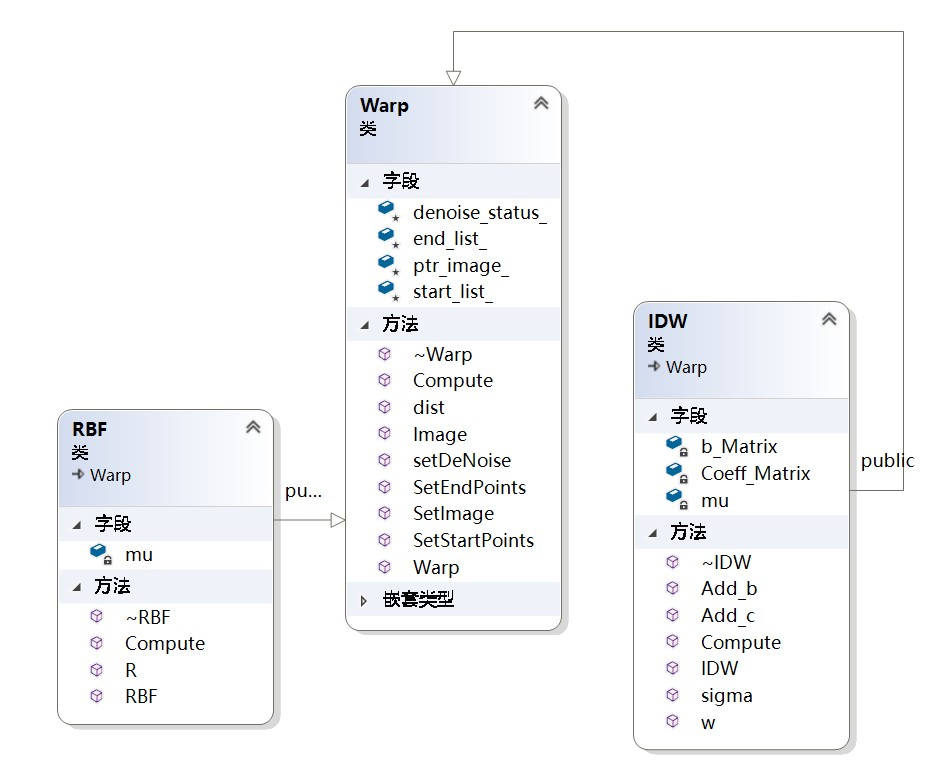
\includegraphics[width=7in]{class1.jpg}
		\end{center}
	\end{figure}
	\clearpage
	\begin{figure}[htb]
		\begin{center}
			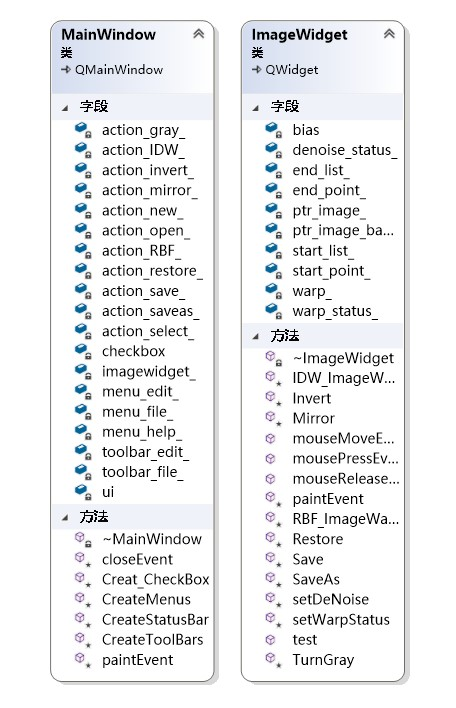
\includegraphics[width=6in]{class2.jpg}
		\end{center}
	\end{figure}
	\clearpage
	\section{实现结果}
	\subsection{UI设计}
	\begin{figure}[htb]
		\begin{center}
		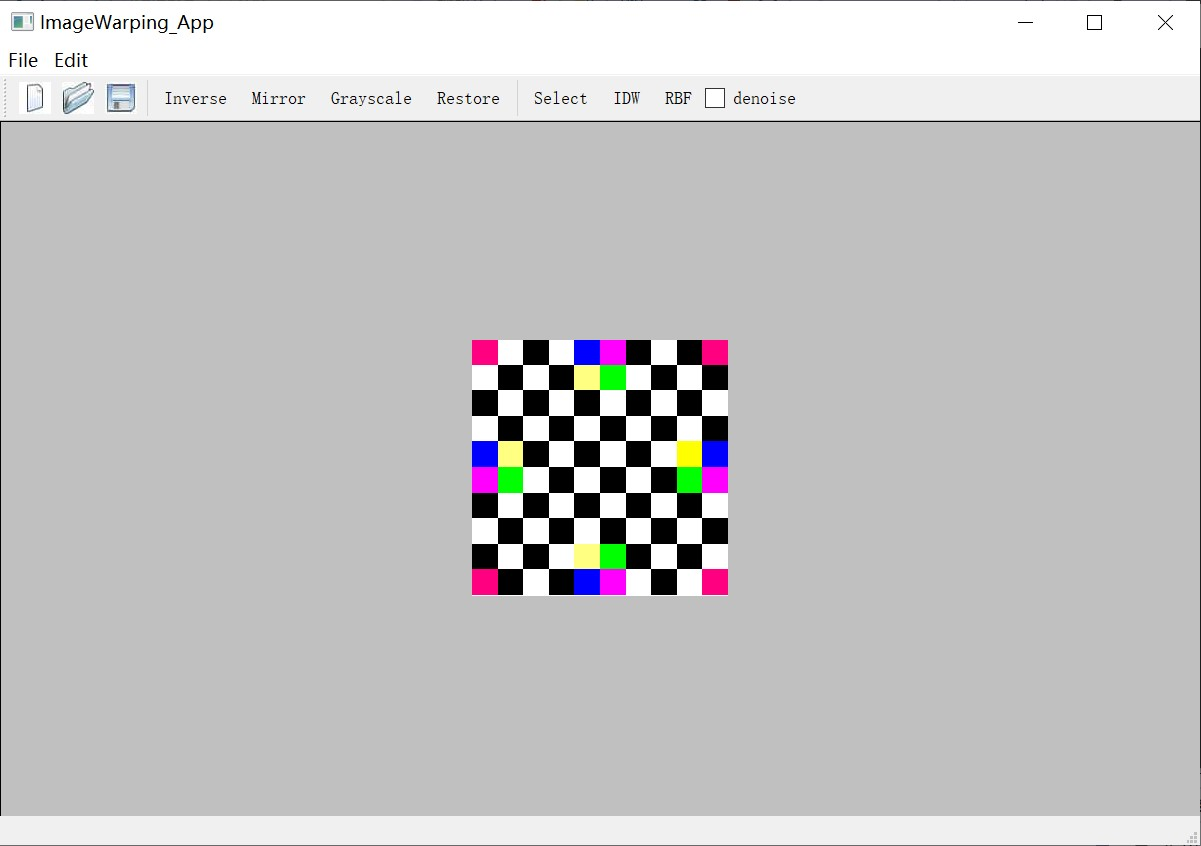
\includegraphics[width=4in]{ui.jpg}
		\end{center}
	\end{figure}
	如上图。点击Select键后可以开始选择控制点(蓝色)和目标点(绿色),鼠标左键点击会画出控
	制点,
	再释放
	就可以画出目标点(如下图)。之后可点击"IDW"键或"RBF"来进行图像变形。复选框用于选择
	是否去噪。
	\begin{figure}[htb]
		\begin{center}
			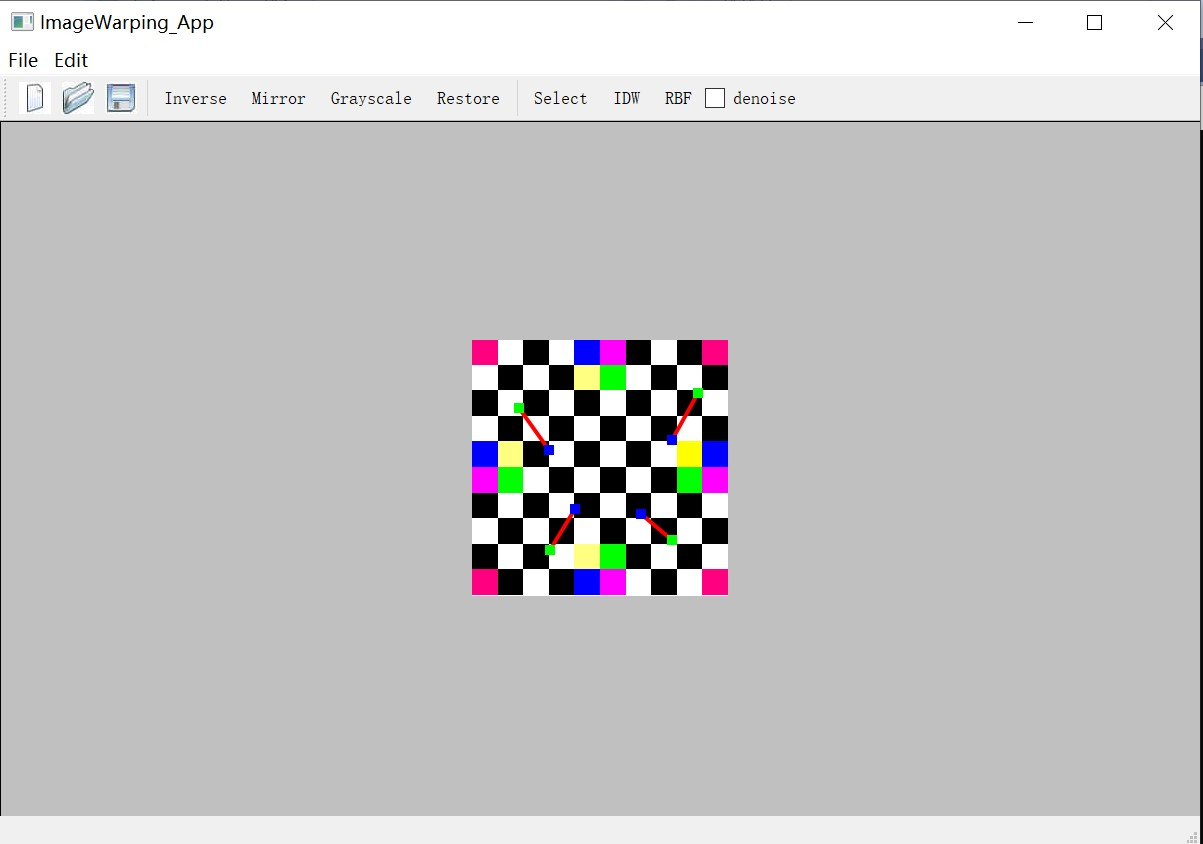
\includegraphics[width=4in]{ui1.jpg}
		\end{center}
	\end{figure}
	\clearpage
	\subsection{变形效果}
	\begin{figure}[htbp]
		\centering
		\begin{minipage}{0.4\linewidth}
			\centering
			\caption{IDW}
			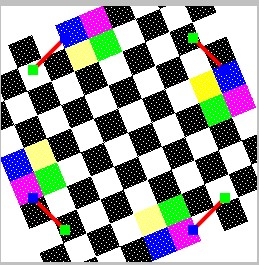
\includegraphics[width=1\linewidth]{IDW1.jpg}
			\label{chutian1}
		\end{minipage}
		%\qquad
		\begin{minipage}{0.4\linewidth}
			\centering
			\caption{RBF}
			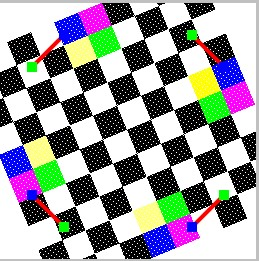
\includegraphics[width=1\linewidth]{RBF1.jpg}
			\label{chutian2}
		\end{minipage}
	\end{figure}
	\begin{figure}[htbp]
		\centering
		\begin{minipage}{0.4\linewidth}
			\centering
			\caption{IDW}
			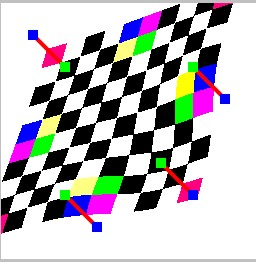
\includegraphics[width=1\linewidth]{IDW2.jpg}
			\label{chutian1}
		\end{minipage}
		%\qquad
		\begin{minipage}{0.4\linewidth}
			\centering
			\caption{RBF}
			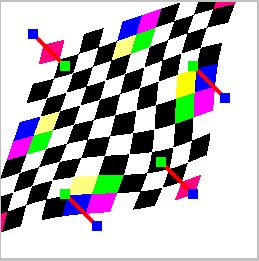
\includegraphics[width=1\linewidth]{RBF2.jpg}
			\label{chutian2}
		\end{minipage}
	\end{figure}
	\clearpage
	\begin{figure}[htbp]
		\centering
		\begin{minipage}{0.4\linewidth}
			\centering
			\caption{IDW}
			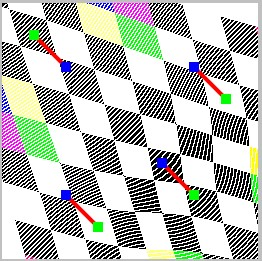
\includegraphics[width=1\linewidth]{IDW3.jpg}
			\label{chutian1}
		\end{minipage}
		%\qquad
		\begin{minipage}{0.4\linewidth}
			\centering
			\caption{RBF}
			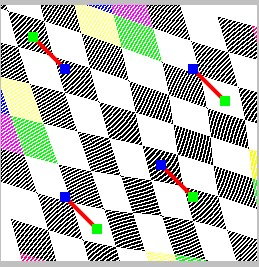
\includegraphics[width=1\linewidth]{RBF3.jpg}
			\label{chutian2}
		\end{minipage}
	\end{figure}
	
	我们可以看到2种方法效果接近,但是都有噪声的出现,或者说裂缝。所以我们这里采用求插值
	函数的逆函数的方法来解决这一问题。但是求插值函数的逆函数相当复杂,所以这里考虑将控
	制点和目标点对调后的插值函数可以近似地作为插值函数的逆函数。实现效果如下:
		\begin{figure}[htbp]
		\centering
		\begin{minipage}{0.4\linewidth}
			\centering
			\caption{IDW}
			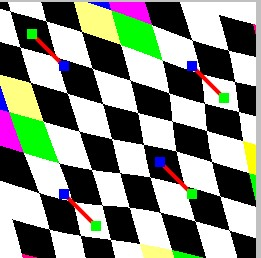
\includegraphics[width=1\linewidth]{IDWde.jpg}
			\label{chutian1}
		\end{minipage}
		%\qquad
		\begin{minipage}{0.4\linewidth}
			\centering
			\caption{RBF}
			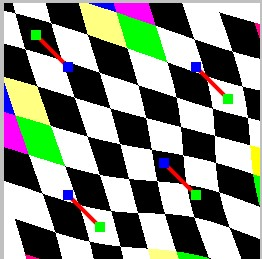
\includegraphics[width=1\linewidth]{RBFde.jpg}
			\label{chutian2}
		\end{minipage}
	\end{figure}

	\section{不足}
	没有采用插值的方法来补缝。
\section{参考文献}
  $[1]$Ruprecht D, Muller H. [**Image warping with scattered data 
  interpolation**]IEEE Computer Graphics and Applications, 1995, 15(2): 37-43.
  
  $[2]$Arad N, Reisfeld D. [**Image warping using few anchor points and radial 
  functions**][C]//Computer graphics forum. Edinburgh, UK: Blackwell Science 
  Ltd, 1995, 14(1): 35-46.
\end{document}
